% Modelo de trabajos del EIMAT 2025 creado por el profesor Gustavo Quintero
% Cualquier error o duda con la compilación de este modelo puede comunicarse al email eimat@matua.edu.co
% NO CREAR CARPETAS NI ARCHIVOS NUEVOS (COMO bibliografia.bib).
% SI NECESITA AGREGAR PAQUETES, COLOQUELOS EN "PAQUETES NUEVOS DEL USUARIO"

\documentclass[11pt]{article}
\usepackage[utf8]{inputenc}
\usepackage[spanish]{babel}
\addto\captionsspanish{\renewcommand{\tablename}{Tabla}}
\usepackage{amsmath}
\usepackage{amsthm}
\usepackage{amsfonts}
\usepackage{hyperref}	
\usepackage{graphicx}
\usepackage{geometry}
\usepackage{fancyhdr}
\usepackage{lmodern}
\usepackage{titling}
\decimalpoint

\setlength{\textwidth}     {16.0cm}
\setlength{\textheight}    {21.0cm}
\setlength{\evensidemargin}{ 0.0cm}
\setlength{\oddsidemargin} { 0.0cm}
\setlength{\topmargin}     {-0.5cm}
\setlength{\baselineskip}  { 0.7cm}

\newtheorem{teorema}{Teorema}
\newtheorem{corolario}{Corolario}
\newtheorem{lema}{Lema}
\newtheorem{definicion}{Definición}

% PAQUETES NUEVOS DEL USUARIO

\begin{document}

\noindent

\begin{center}
\Large\bf{XXII Encuentro Internacional de Matem\'{a}ticas 
EIMAT 2026}
\end{center}

\vspace{1cm}

% COLOQUE AQUÍ EL TITULO DE SU TRABAJO
\begin{center}
\Large\bf{Titulo del trabajo}
\end{center}

\vspace{0.5cm}

% COLOQUE AQUÍ LOS DATOS DEL AUTOR (O AUTORES SI HAY MAS DE UNO)
\begin{center}
\textbf{Gustavo David Quintero Álvarez}\\
Universidad del Atlántico\\
\emph{E-mail: eimat@matua.edu.co}
\end{center}

% SI NO HAY MAS AUTORES BORRE ESTA PARTE
\begin{center}
\textbf{Nombre completo segundo autor}\\
Institución\\
\emph{E-mail: autor2@dominio.edu.co}
\end{center}

\vspace{0.5cm}
\section*{Resumen}
% ESPACIO PARA EL RESUMEN DEl TRABAJO NO MAYOR A 4500 CARACTERES EN PONENCIAS O PÓSTER Y 8000 PARA CURSILLOS.
La integral de Riemann es una formalización del proceso de hallar el área bajo una curva sobre un intervalo cerrado \( [a, b] \). Consiste en aproximar esta área mediante sumas de áreas de rectángulos construidos a partir de particiones del intervalo (\cite{bartle2000, apostol1974}). Se dice que una función \( f:~[a,b] \to \mathbb{R} \) es integrable en el sentido de Riemann si existe un número real \( I \) tal que, para toda partición suficientemente fina del intervalo y cualquier elección de puntos intermedios, las sumas de Riemann se aproximan a \( I \), para mas detalles consulte \cite{rudin1976}. Una condición suficiente para la integrabilidad de \( f \) en \( [a,b] \) es que sea continua o que tenga un número finito de discontinuidades. 

\begin{definicion}
Una partición \( \mathcal{P} \) del intervalo \( [a,b] \) es un conjunto finito de puntos
\[
\mathcal{P} = \{ x_0, x_1, \dots, x_n \}
\]
tal que \( a = x_0 < x_1 < \dots < x_n = b \).
\end{definicion}

\begin{definicion}
Para cada subintervalo \( [x_{i-1}, x_i] \), definimos:
\[
m_i = \inf \{ f(x) : x \in [x_{i-1}, x_i] \}, \quad M_i = \sup \{ f(x) : x \in [x_{i-1}, x_i] \}
\]
Entonces, la suma inferior y suma superior de \( f \) respecto a la partición \( \mathcal{P} \) son:
\[
L(f, \mathcal{P}) = \sum_{i=1}^n m_i (x_i - x_{i-1}), \quad U(f, \mathcal{P}) = \sum_{i=1}^n M_i (x_i - x_{i-1})
\]
\end{definicion}

\begin{definicion}
Se define la \emph{integral inferior} y \emph{superior} de \( f \) como:
\[
\underline{\int_a^b} f(x)\,dx = \sup_{\mathcal{P}} L(f, \mathcal{P}), \quad 
\overline{\int_a^b} f(x)\,dx = \inf_{\mathcal{P}} U(f, \mathcal{P})
\]
\end{definicion}

Decimos que \( f \) es integrable en el sentido de Riemann (ver \cite{royden1988}) si:
\[
\underline{\int_a^b} f(x)\,dx = \overline{\int_a^b} f(x)\,dx
\]
y en ese caso, el valor común se denota por
\[
\int_a^b f(x)\,dx
\]

\begin{figure}[ht!]
    \centering
    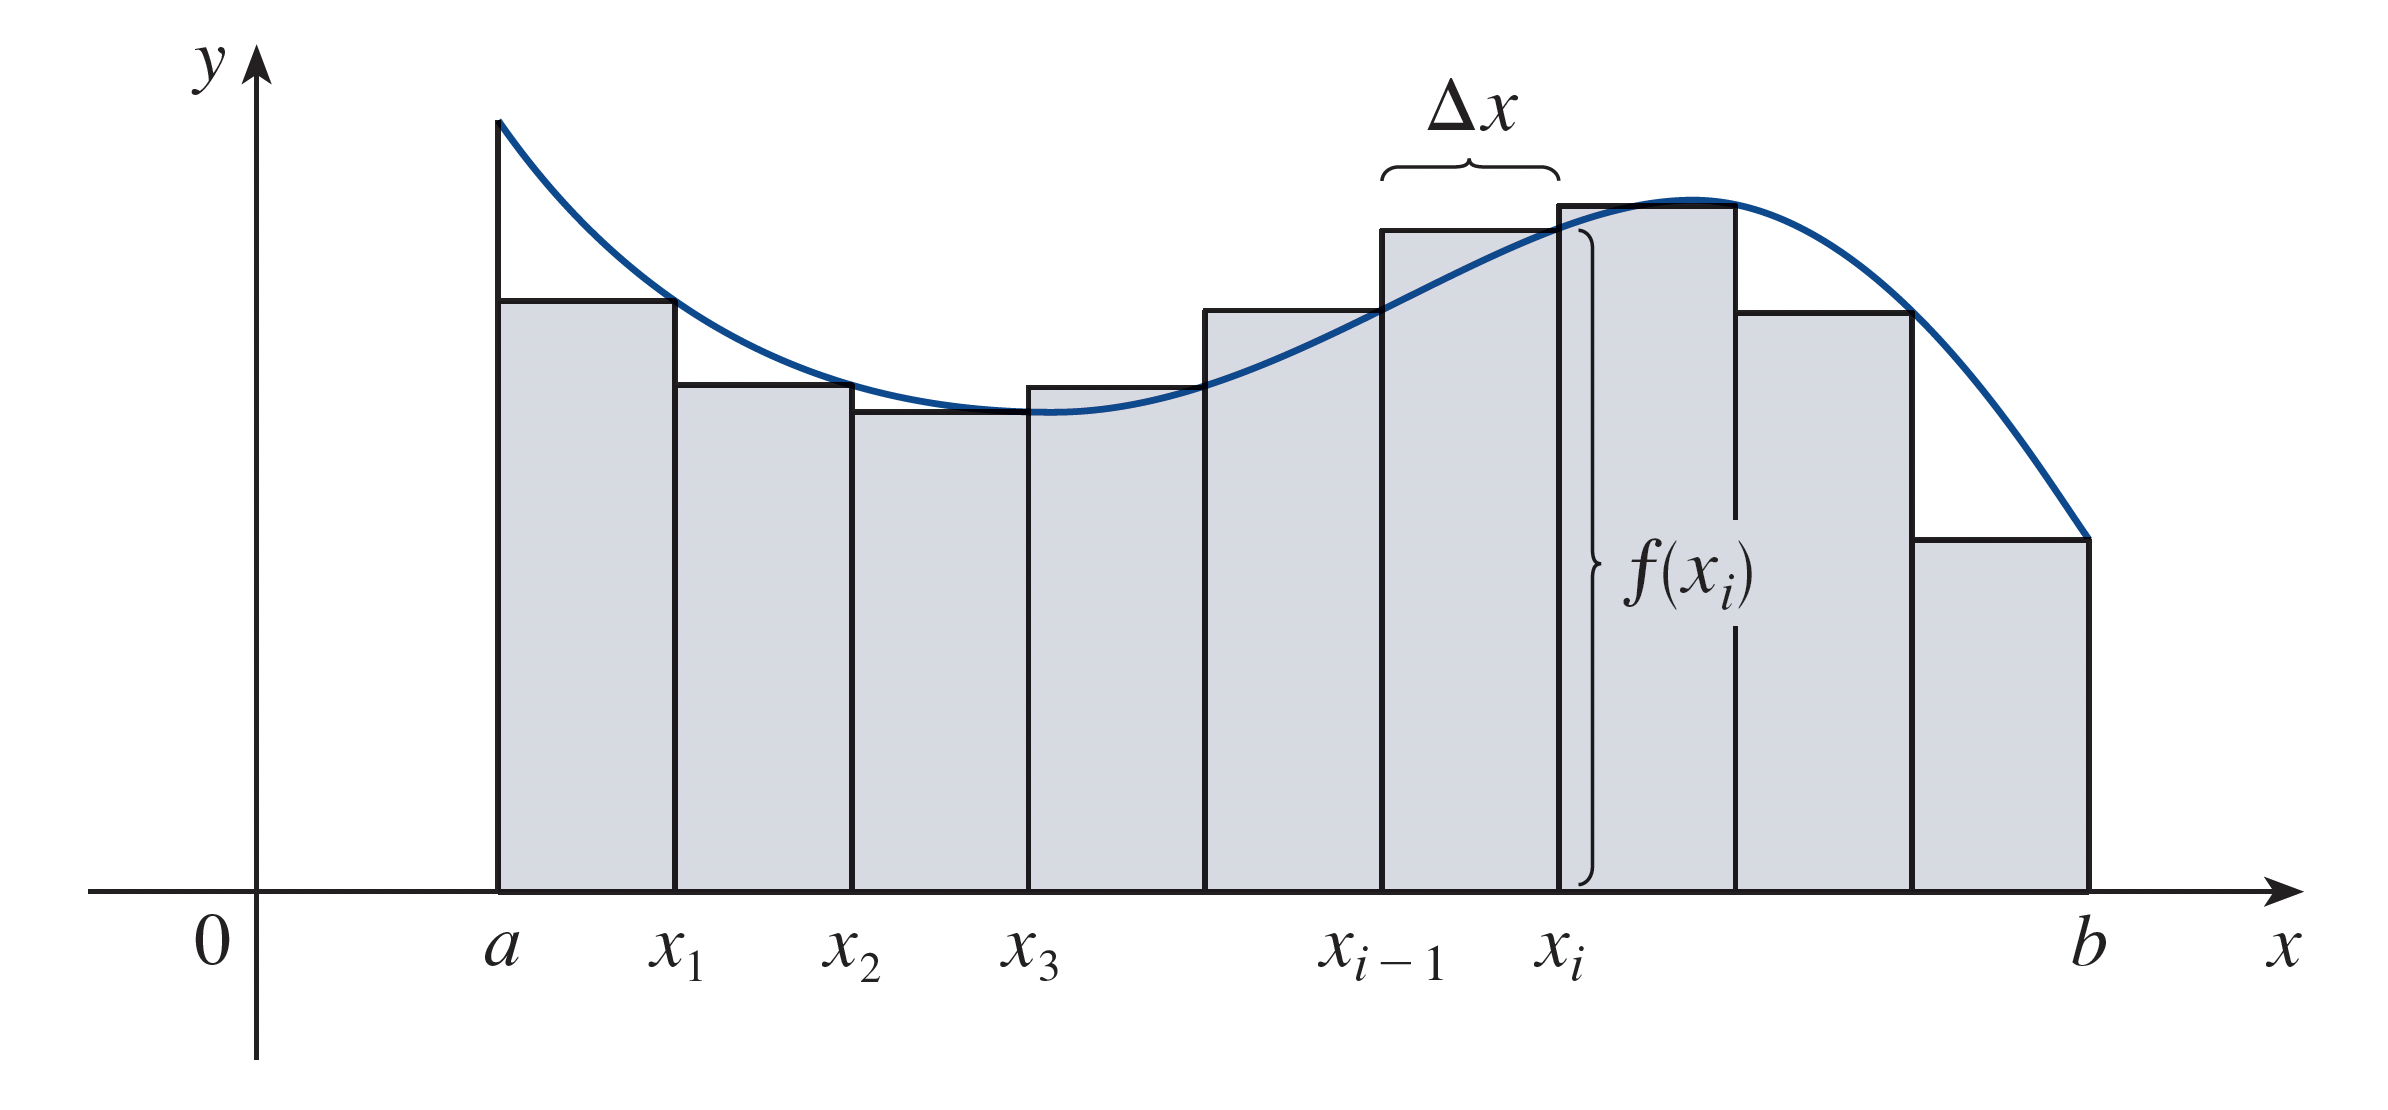
\includegraphics[width=0.8\linewidth]{image.png}
    \caption{Imagen en \LaTeX}
    \label{fig:integral}
\end{figure}

\begin{teorema}
Toda función continua en \( [a,b] \) es integrable en el sentido de Riemann. Más generalmente, si \( f \) es acotada y el conjunto de sus discontinuidades tiene medida de Lebesgue nula (en particular, si tiene un número finito de discontinuidades), entonces \( f \) es Riemann-integrable.
\end{teorema}

\begin{proof}
Ver \cite{rudin1976}.
\end{proof}

Ejemplo de citación de articulo científico: ~\cite{paper}.\\

\begin{table}[ht!]
    \centering
    \begin{tabular}{|c|c|c|c|}
    \hline
    Columna 1 & Columna 2 & Columna 3 & Columna 4 \\
    \hline\hline
    0.847 & 0.123 & 0.562 & 0.391 \\
    0.274 & 0.935 & 0.081 & 0.746 \\
    0.619 & 0.458 & 0.307 & 0.924 \\
    0.183 & 0.772 & 0.645 & 0.039 \\
    0.521 & 0.264 & 0.889 & 0.417 \\
    \hline
    \end{tabular}
    \caption{Ejemplo de una tabla en \LaTeX}
    \label{etiqueta}
\end{table}

\noindent
\textbf{Palabras Clave:} Palabra clave 1, Palabra clave 2, etc.

\begin{thebibliography}{99}

\bibitem{bartle2000}
R.~G. Bartle and D.~R. Sherbert, \emph{Introduction to Real Analysis}, \textit{Wiley}, 3rd edition, 2000.

\bibitem{apostol1974}
T.~M. Apostol, \emph{Mathematical Analysis}, \textit{Addison-Wesley}, 2nd edition, 1974.

\bibitem{rudin1976}
W.~Rudin, \emph{Principles of Mathematical Analysis}, \textit{McGraw-Hill}, 3rd edition, 1976.

\bibitem{royden1988}
H.~L. Royden, \emph{Real Analysis}, \textit{Macmillan}, 3rd edition, 1988.

\bibitem{paper} E. G. Birgin and J. M. Mart\'{\i}nez, Complexity and performance of an Augmented Lagrangian algorithm, \textit{Optimization Methods and Software} 35, pp. 885--920, 2020.

\end{thebibliography}

\end{document}
